%%%%%%%%%%%%%%%%%%%%%%%%%%%%%%%%%%%%%%%%%%%%%%%%%%%%%%%%%%%%%%%

% Document Header %

% Importing Libraries %
\documentclass[12pt, a4paper,openany]{article}
\usepackage{caption}
\usepackage{titlesec}
\usepackage{subcaption}
\usepackage[utf8]{inputenc}
\usepackage{amsmath} 

\usepackage{graphicx} 
\usepackage[a4paper, total={6in, 9in}]{geometry}
\usepackage{titling}

\usepackage{tikz}
\usetikzlibrary{shapes.geometric, arrows}
\usetikzlibrary{positioning}
\usetikzlibrary{calc}
% Defining Defaults %
\usepackage[table,xcdraw]{xcolor}
\graphicspath{{Images/}}
\titlespacing*{\section}{0pt}{-1pt}{1.5\baselineskip}
\titlespacing*{\subsection}{0pt}{*1}{1.0\baselineskip}
% Defining tikzstyle for Flow Charts %
\tikzstyle{ghost} = [rectangle, 
minimum width=1.5cm, 
minimum height=1cm, 
text centered, 
text width=1cm, 
draw=black!0 
]
\tikzstyle{startstop} = [rectangle, rounded corners, 
minimum width=3cm, 
minimum height=1cm,
text centered, 
text width = 5cm,
draw=black, 
fill=red!20]

\tikzstyle{startstop_o} = [rectangle, rounded corners, 
minimum width=3cm, 
minimum height=1cm,
text centered, 
text width = 5cm,
draw=black, 
fill=orange!20]

\tikzstyle{startstop_c} = [rectangle, rounded corners, 
minimum width=3cm, 
minimum height=1cm,
text centered, 
text width = 5cm,
draw=black, 
fill=green!20]

\tikzstyle{startstop_cy} = [rectangle, rounded corners, 
minimum width=3cm, 
minimum height=1cm,
text centered, 
text width = 5cm,
draw=black, 
fill=cyan!20]

\tikzstyle{startstop_y} = [rectangle, rounded corners, 
minimum width=3cm, 
minimum height=1cm,
text centered, 
text width = 5cm,
draw=black, 
fill=yellow!20]


\tikzstyle{startstop_w} = [rectangle, rounded corners, 
minimum width=3cm, 
minimum height=1cm,
text centered, 
text width = 6cm,
draw=black, 
fill=red!20]

\tikzstyle{startstop_wg} = [rectangle, rounded corners, 
minimum width=3cm, 
minimum height=1cm,
text centered, 
text width = 6cm,
draw=black, 
fill=green!20]

\tikzstyle{startstop_wb} = [rectangle, rounded corners, 
minimum width=3cm, 
minimum height=1cm,
text centered, 
text width = 6cm,
draw=black, 
fill=blue!20]

\tikzstyle{startstop_wr} = [rectangle, rounded corners, 
minimum width=3cm, 
minimum height=1cm,
text centered, 
text width = 6cm,
draw=black, 
fill=red!20]

\tikzstyle{process} = [rectangle, 
minimum width=3cm, 
minimum height=1cm, 
text centered, 
text width=5cm, 
draw=black, 
fill=orange!30]

\tikzstyle{process_c} = [rectangle, 
minimum width=3cm, 
minimum height=1cm, 
text centered, 
text width=5cm, 
draw=black, 
fill=cyan!30]


\tikzstyle{process_small} = [rectangle, 
minimum width=3cm, 
minimum height=1cm, 
text centered, 
text width=4cm, 
draw=black, 
fill=orange!30]

\tikzstyle{process_smallc} = [rectangle, 
minimum width=3cm, 
minimum height=1cm, 
text centered, 
text width=4cm, 
draw=black, 
fill=cyan!30]

\tikzstyle{process_wide} = [rectangle, 
minimum width=3cm, 
minimum height=1cm, 
text centered, 
text width=6cm, 
draw=black, 
fill=orange!30]

\tikzstyle{process_widec} = [rectangle, 
minimum width=3cm, 
minimum height=1cm, 
text centered, 
text width=6cm, 
draw=black, 
fill=cyan!30]

\tikzstyle{process_uwide} = [rectangle, 
minimum width=3cm, 
minimum height=1cm, 
text centered, 
text width=8cm, 
draw=black, 
fill=orange!30]

\tikzstyle{process_uwidec} = [rectangle, 
minimum width=3cm, 
minimum height=1cm, 
text centered, 
text width=8cm, 
draw=black, 
fill=cyan!30]

\tikzstyle{line} = [draw,-latex]
% Defining Title Sequence %
\title{\vspace{-3cm} \makebox[\textwidth][c]{COL215 SW Assignment 1 - Gate Packing}}
\author{Submission By :\\ \hspace{0.5cm} \textbf{Yash Rawat} \hspace{1cm} \textbf{Priyanshi Gupta}\\ \textbf{2023CS50334} \hspace{1.3cm} \textbf{2023CS10106} \\ \\ Department of Computer Science and Engineering \\ Indian Institute of Technology, Delhi}
\date{\today}
% Ending Document Header %

%%%%%%%%%%%%%%%%%%%%%%%%%%%%%%%%%%%%%%%%%%%%%%%%%%%%%%%%%%%%%%%
% Starting document Page 1%
%%%%%%%%%%%%%%%%%%%%%%%%%%%%%%%%%%%%%%%%%%%%%%%%%%%%%%%%%%%%%%%
\begin{document} 
\maketitle

% B_Roll For Project in Minipage Env %
\begin{figure}[ht]
\centering
  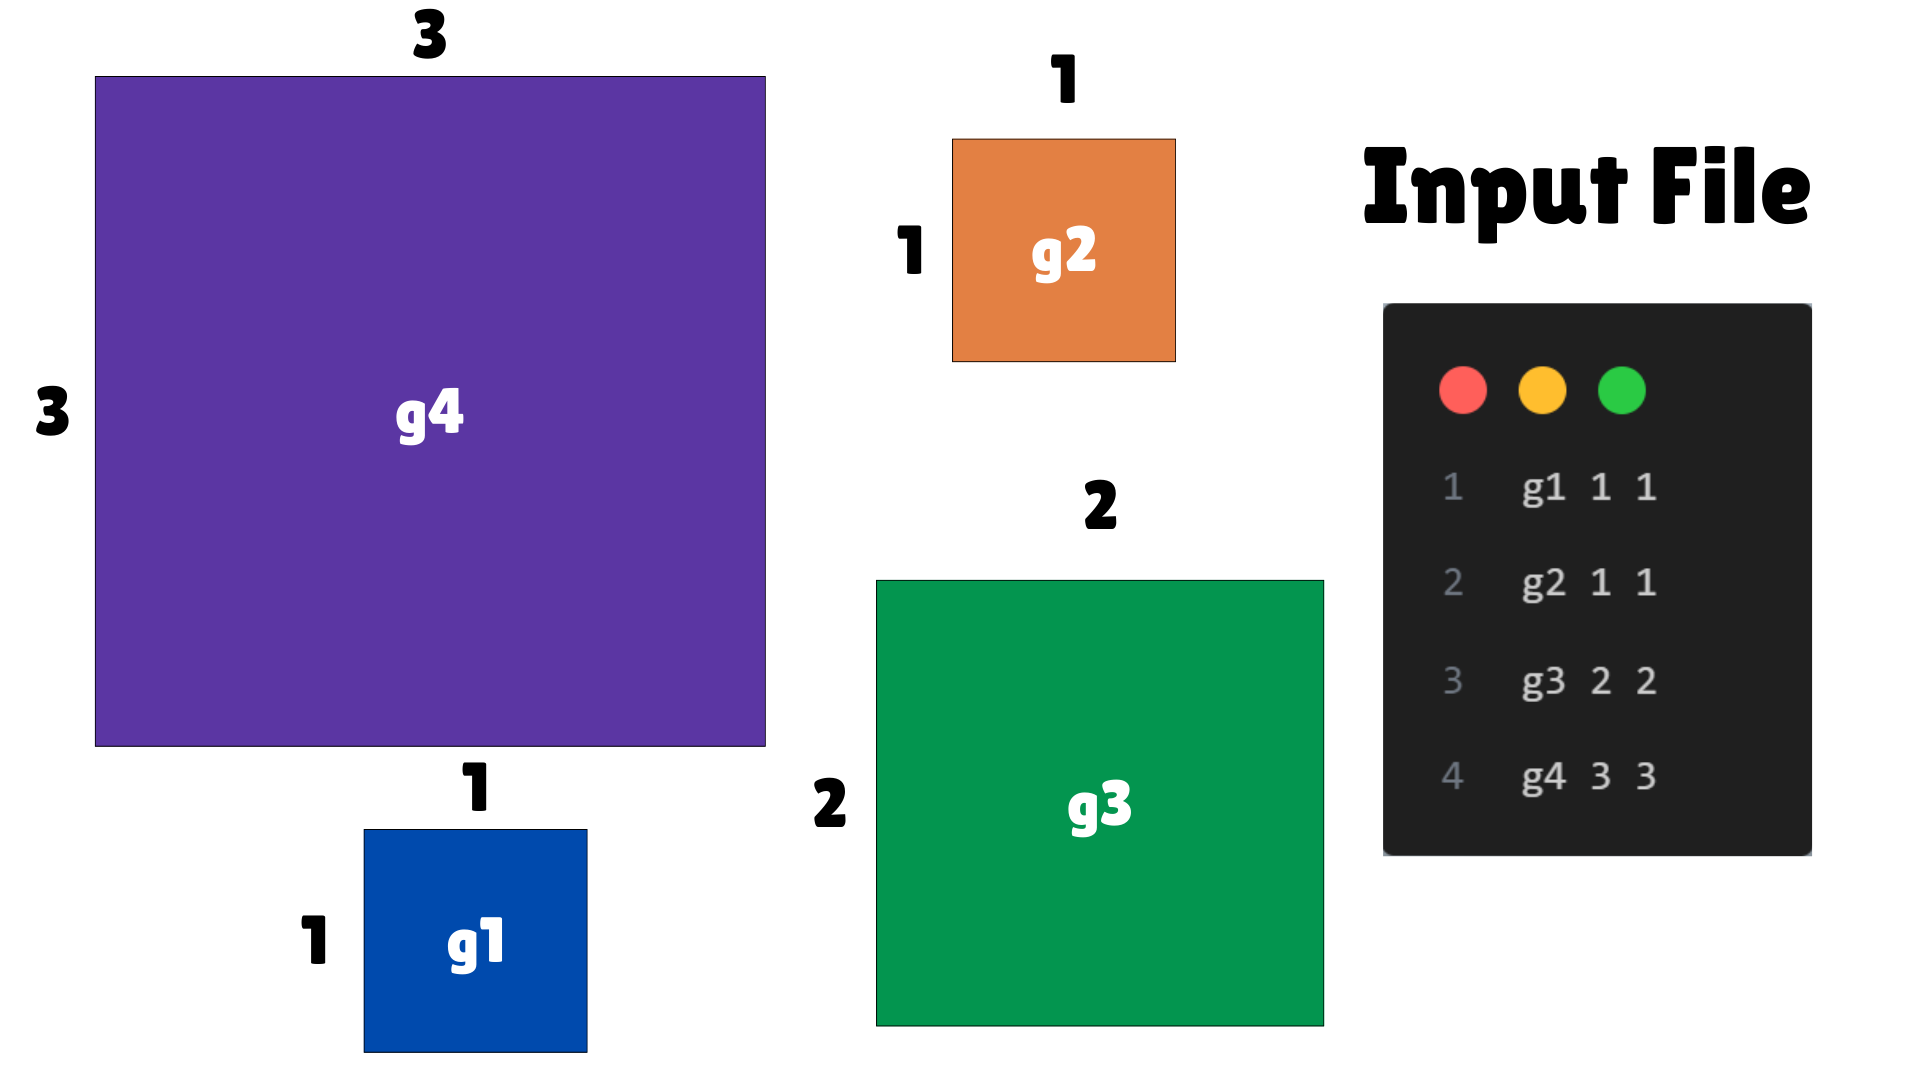
\includegraphics[width=0.8\linewidth]{BRoll/tc1_rep}
  % \captionof{figure}{A figure}
  \label{fig:basys_b}
\end{figure}
\begin{figure}[ht]
  \centering
  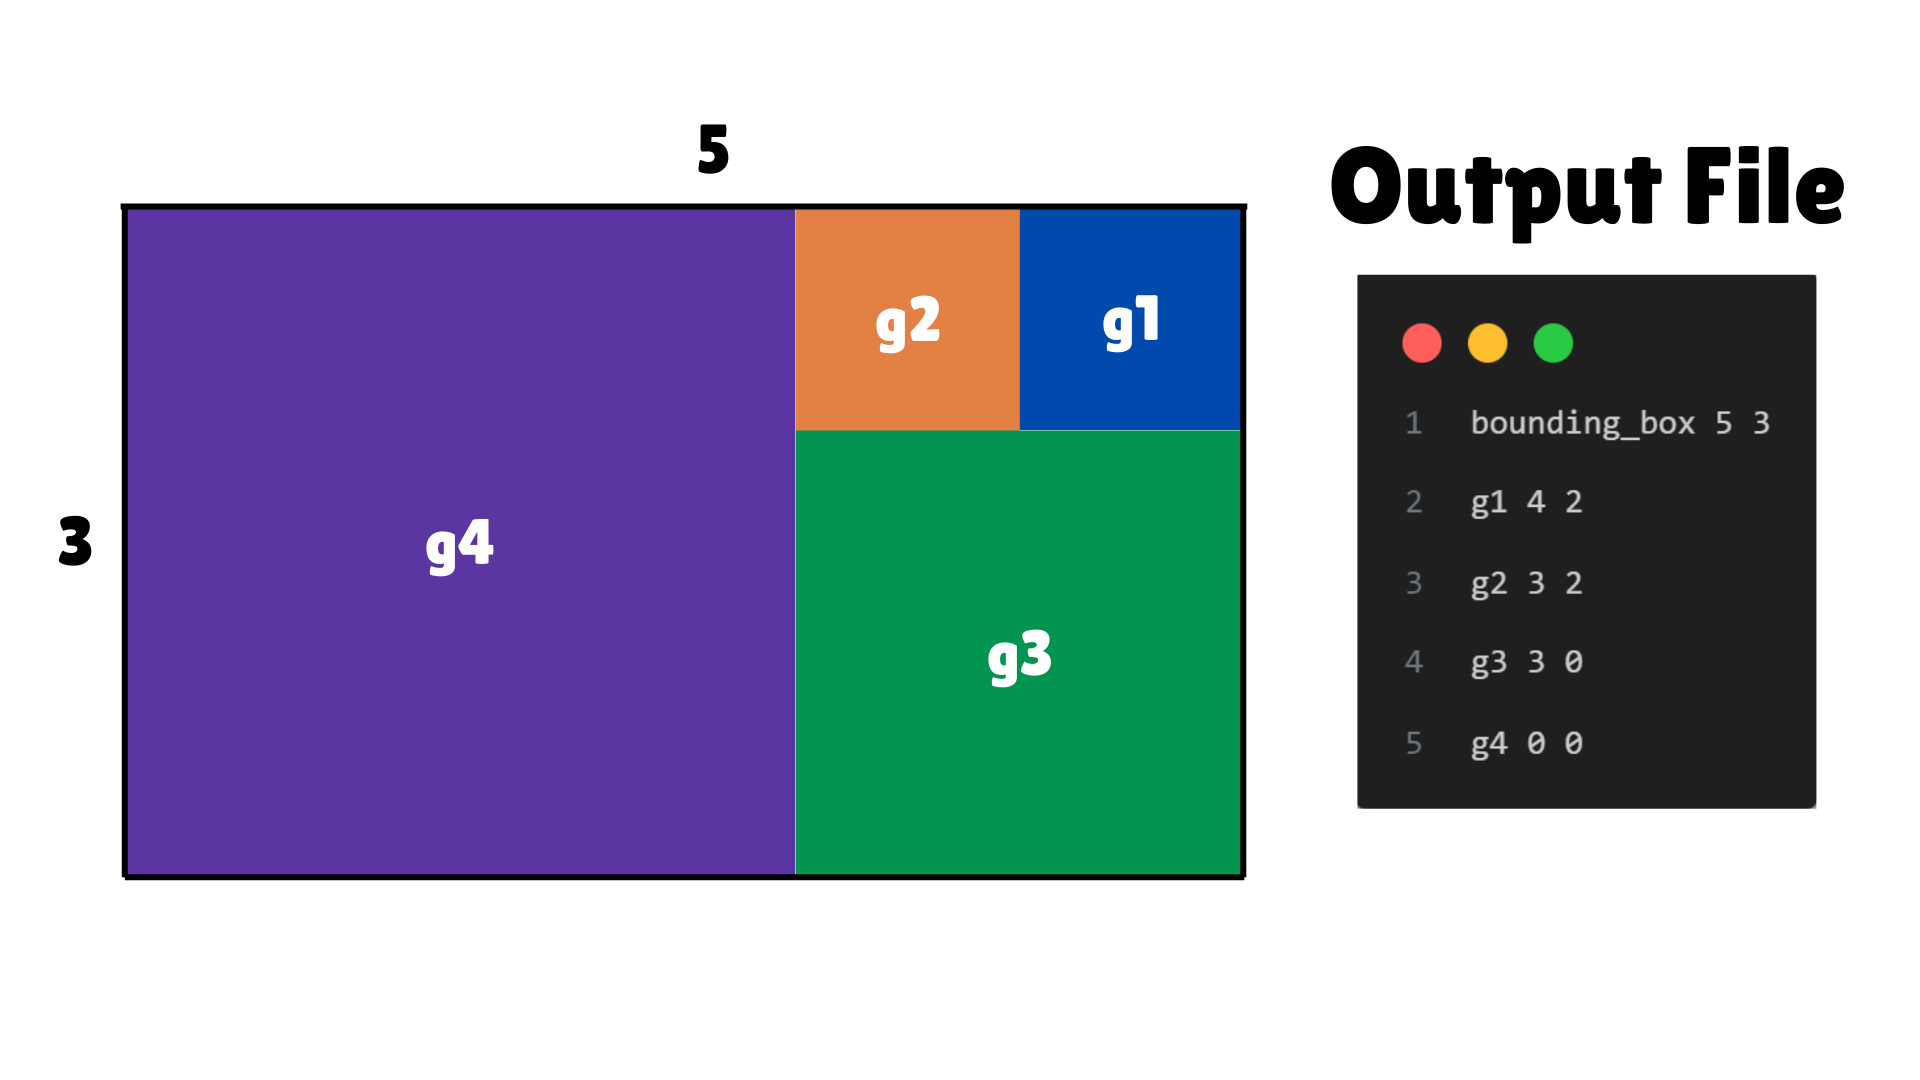
\includegraphics[width=0.8\linewidth]{BRoll/tc1_out_rep}
  % \captionof{figure}{Another figure}
  \label{fig:broll_mux}
\end{figure}

%%%%%%%%%%%%%%%%%%%%%%%%%%%%%%%%%%%%%%%%%%%%%%%%%%%%%%%%%%%%%%%
\newpage % Begin Page 2 %
%%%%%%%%%%%%%%%%%%%%%%%%%%%%%%%%%%%%%%%%%%%%%%%%%%%%%%%%%%%%%%%

\section{Modelling Gate Packing}
\subsection{What is Gate Packing ?}
\begin{flushleft}
In the context of gate level circuit designing, it refers to the process of arranging logic gates on a circuit board in order to minimize wasted space, reduce interconnection length and optimize the overall layout of the circuit board.
\end{flushleft}
\begin{flushleft}
Generalised gate packing is a very complex problem and involves multiple challenges such as placement and routing complexity, heat dissipation, design constraints due to fabrication processes, etc. but we will be tackling a simplified problem in this assignment.
\end{flushleft}
\subsection{Understanding the Problem Statement}
\begin{flushleft}
The problem statement models the gates as a set of n rectangles (provided as input for each test case) : \( \{g_{1},g_{2},...,g_{n}\}\) each represented by a pair of integers : \(g_{i} = (w_{i},h_{i})\) , where \(w_{i}\) and \(h_{i}\) are the width and the height of the \(i^{th}\) board. A given set of gates is said to be “correctly assigned" if no two gates have overlapping areas. The bounding rectangle is defined to be the smallest rectangle that encloses all gates and has the minimum area (out of all the possible “correctly assigned" cases).
\end{flushleft}

\begin{flushleft}
The program is supposed to output 2 things - The \(w\) and \(h\) of the bounding rectangle and the set of coordinates : \(\{ (x_{i},y_{i})\}^{i=n}_{i=1}\) - where \((x_{i},y_{i})\) denote the coordinate of the bottom left corner of the \(g_{i}\). A sample test case is given below :
(Note that every gate placed is in the original orientation provided by test case, i.e. re-orientation by rotation is disallowed)
\end{flushleft}

\begin{figure}[ht]
\centering
  \includegraphics[width=0.75\linewidth]{BRoll/tc2_rep}
  % \captionof{figure}{A figure}
   \label{fig:TC2}
   \captionof{figure}{Sample Test Case with 8 gates}
\end{figure}

%%%%%%%%%%%%%%%%%%%%%%%%%%%%%%%%%%%%%%%%%%%%%%%%%%%%%%%%%%%%%%%
% Begin Page 3 %
%%%%%%%%%%%%%%%%%%%%%%%%%%%%%%%%%%%%%%%%%%%%%%%%%%%%%%%%%%%%%%%

\begin{figure}[ht]
  \centering
  \includegraphics[width=0.75\linewidth]{BRoll/tc2_out_rep}
  % \captionof{figure}{Another figure}
  \label{fig:TC2_OUT}
  \captionof{figure}{Output of above sample case}
\end{figure}

\section{Algorithm Conceptualization and Design}
\begin{flushleft}
Our all three Algorithms solve the problem in a Y Direction Flipped manner.
Since the \((0,0)\) of our grid co-ordinates are taken in the top left (allowing us to iterate the grid in row-major order)
(which is different from the given problem statement where \((0,0)\) is taken in bottom right). Hence if any
correct packing is found by our algorithm then it will also work in the original problem statement.
\end{flushleft}
\begin{figure}[ht]
  \centering
  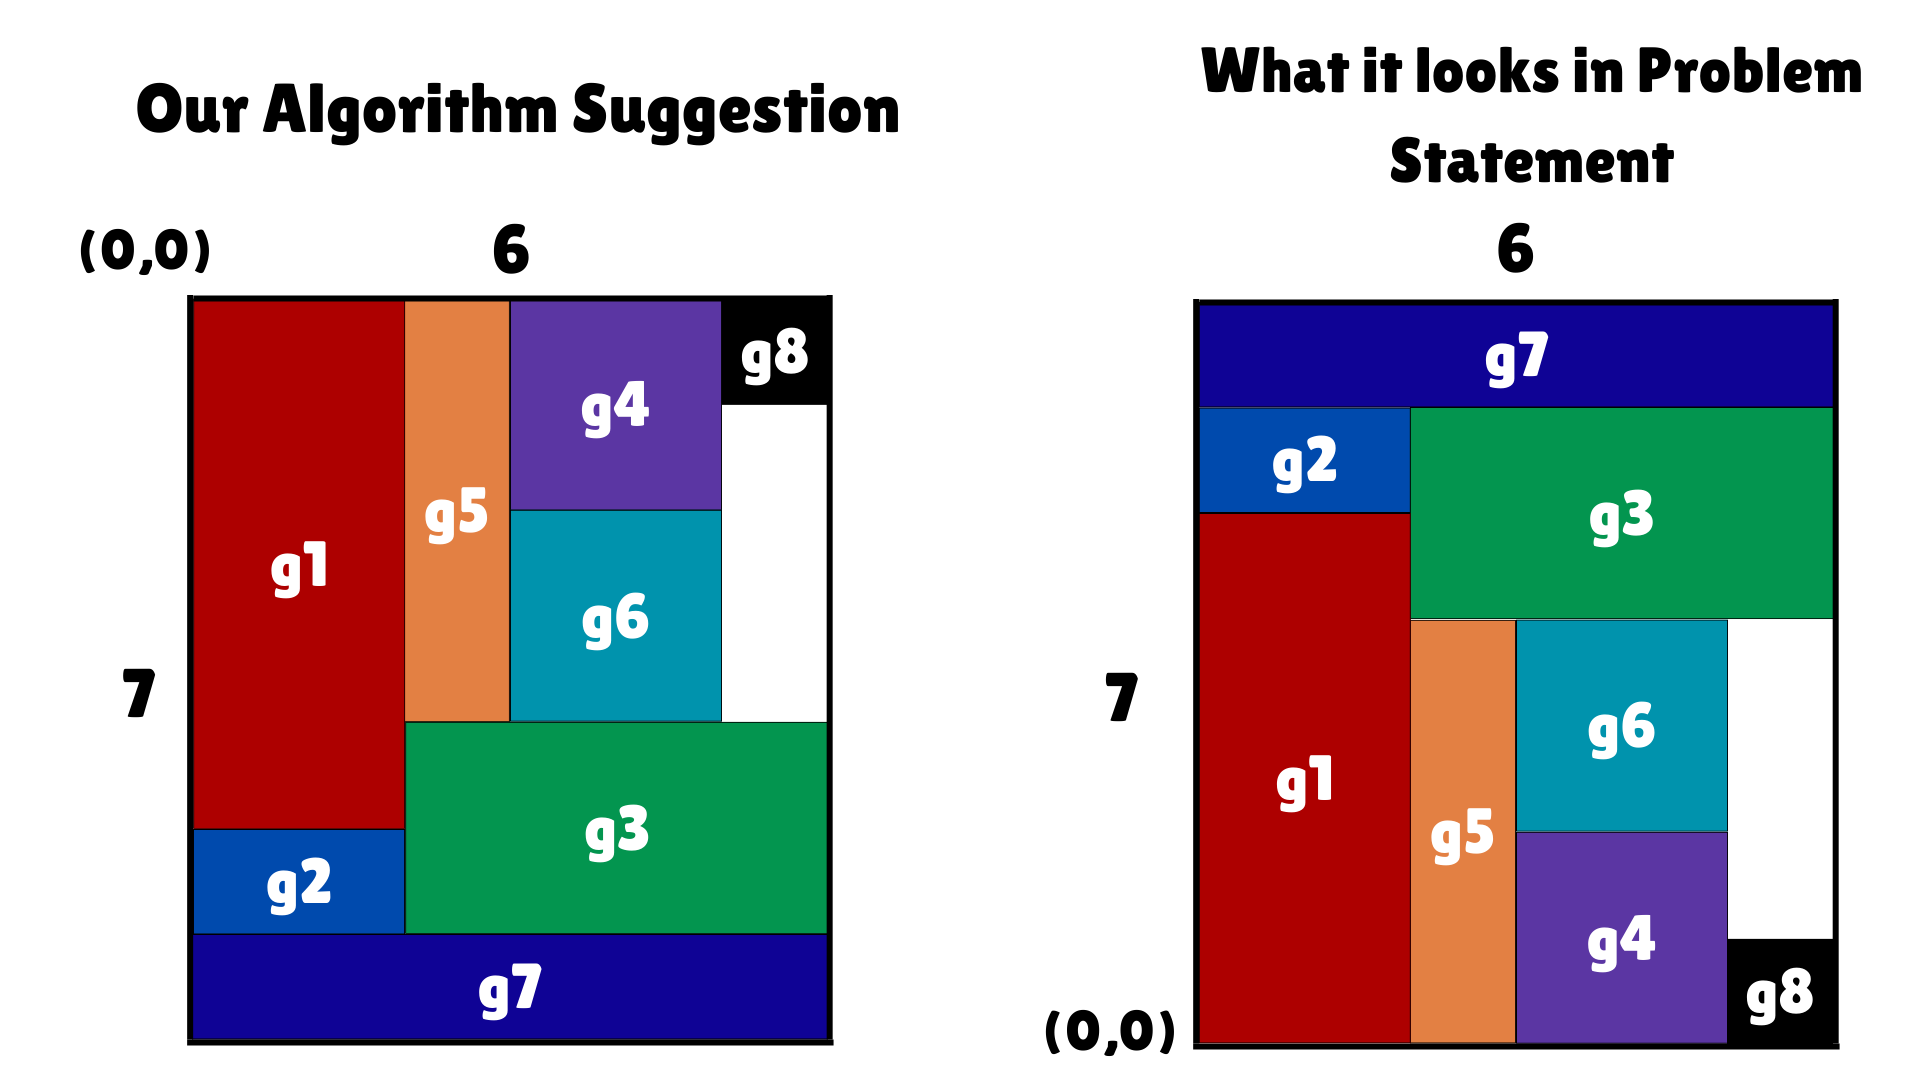
\includegraphics[width=0.8\linewidth]{BRoll/TC_Compare.png}
  % \captionof{figure}{Another figure}
  \label{fig:TC_Compare}
  \captionof{figure}{Y Flipped Output by our Algorithm}
\end{figure}

%%%%%%%%%%%%%%%%%%%%%%%%%%%%%%%%%%%%%%%%%%%%%%%%%%%%%%%%%%%%%%%
\newpage % Begin Page 4 %
%%%%%%%%%%%%%%%%%%%%%%%%%%%%%%%%%%%%%%%%%%%%%%%%%%%%%%%%%%%%%%%
\subsection{Naive Row Packing Algorithm}
\begin{flushleft}
This is a naive and one of the simplest ways to pack rectangles and involves following steps :
\begin{enumerate}
    \item Rectangles are sorted in decreasing order of height and width in respective priorities.
    \item Rectangles are added to a row from left to right until next rectangle does not fit.In such case the next rectangle is placed in the next row.
\end{enumerate}
\end{flushleft}


\subsection{Pixel Scan Algorithm}
\begin{flushleft}
The naive row packing algorithm can be improved by manually scanning the entire image for a suitable location for every rectangle to pack. This process would be slower, but that can be improved later on. This is still extremely naive in terms of the actual packing logic.
\begin{enumerate}
    \item Rectangles are sorted in decreasing order of height (and then by width).
    \item The algorithm implements a grid which stores value of every pixel.
    \item We then loop over all our rectangles, and for each one go through every pixel and check if the top left and bottom right of the rectangle (some other pixel) will fit at that location. We also check if this rectangle will go outside the boundary.
    \item  We check all the pixels inside that rectangle to make sure we don’t overlap with some other already placed rectangle.
    \item Once we find a valid location we store location in the rectangle and mark those pixels as occupied in the grid.
    \end{enumerate}
\end{flushleft}

\subsection{Predictive-Pixel Scan Algorithm}
\begin{flushleft}
\begin{enumerate}
    \item The improved algorithm involves sorting rectangles by height (and then by width) just like the previous algorithms.
    \item The algorithm implements a grid which stores 0 for unoccupied pixels and index value i of rectangle which occupies it.
    \item We iterate through the grid but instead of  looping through every pixel and checking its state , we check if a pixel is occupied or not. If it is occupied then we fetch the rectangle width using the index and calculate the nearest column to the right which is not being covered by that rectangle and move our checking coordinates to that column ( same row ).If we exceed the width of image then we just move to the first column of the next row and continue with the iteration.(This step makes the algorithm more efficient).
    \item If empty pixel is returned then the grid is checked to ensure that the next rectangle can be placed in it or not.If it encounters a covered pixel the outer loop is continued(CHECK).
    \item Once we find suitable position for the rectangle it fills the cells with index of the covering rectangle , sets the packed state of rectangle object, as well as its coordinates. 
\end{enumerate}

\end{flushleft}

% Flow Chart tikzpic %
\begin{center}
    

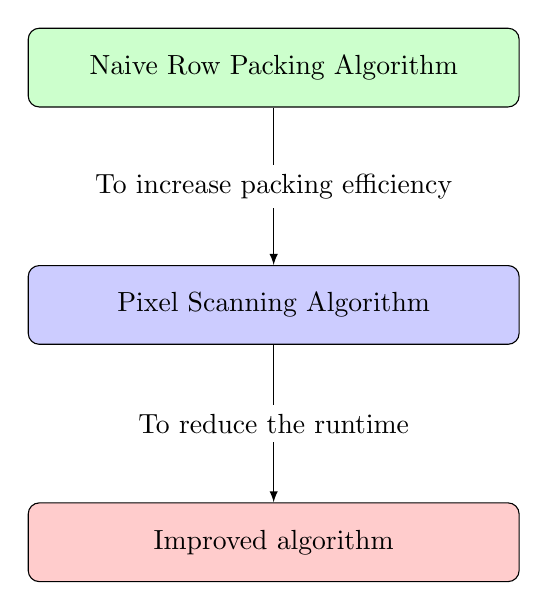
\begin{tikzpicture}[node distance= 2cm and 2cm][ht]

\node [startstop_wg] (s1) {Naive Row Packing Algorithm};
\node [startstop_wb,below = of s1] (s2) {Pixel Scanning Algorithm};
\node [startstop_wr, below = of s2] (s3) {Improved algorithm};

\path [line](s1) -- node[fill = white] {To increase packing efficiency}  (s2);
\path [line](s2) -- node[fill = white] {To reduce the runtime } (s3);

\end{tikzpicture}
\end{center}

\subsection{Proving Correctness of algorithm}

\subsubsection{Selection of Initial Width of Packing}
\begin{enumerate}
    \item The first choice of number of rows and columns in the grid is done by calculating the total area of the rectangles to be packed.Both the height and width are taken to be $\lfloor 1.1 \cdot \sqrt{A} \rfloor$ where A is the total area of gates to be packed.
    \begin{center}
         $W_{0}=\lfloor(1.1\cdot\sqrt{A} \rfloor $
    \end{center}
    \item In case there is no possible packing arrangement we reset the width to 1.5 of width in previous iteration until the packing is done.
    \begin{center}
        $W_{i+1}=\lfloor 1.5 \cdot W_{i} \rfloor$ 
    \end{center}
    \item If we ensure that our rows are more than the maximum height of the gates then this process will terminate in finite steps since a feasible upper bound on the number of columns is the sum of widths of all gates (as in the Naive Row Packing Algorithm).
\end{enumerate}
% Beginning Page 6
\newpage
% Beginning Page 6
\begin{figure}[ht]
    \centering
    \begin{minipage}{.6\textwidth}
          
          \includegraphics[width=1.0\linewidth]{Images/BRoll/annot.jpg}
          % \captionof{figure}{A figure}
          \label{fig:annot-1}
          \caption{Gate Packing }
          
               
    \end{minipage}
\end{figure}


\subsubsection{Optimizing the Algorithm}

After a satisfactory packing arrangement is found we try to find a better arrangement by varying the height and width of the grid.
\begin{enumerate}
    \item We vary the width of the grid in intervals of 2.5\% of initial width and adjust height of grid accordingly.
    \item The time taken and packing efficiency are calculated for the adjusted width and height. A maximum of 20 iterations are carried out to find the best packing.
    \item The iterations stop once packing efficiency exceeds 95\% and runtime is below 2-3 sec.
\end{enumerate}

\newpage
\begin{figure}[ht]
    \centering
    \begin{minipage}{1.0\textwidth}
          \centering
          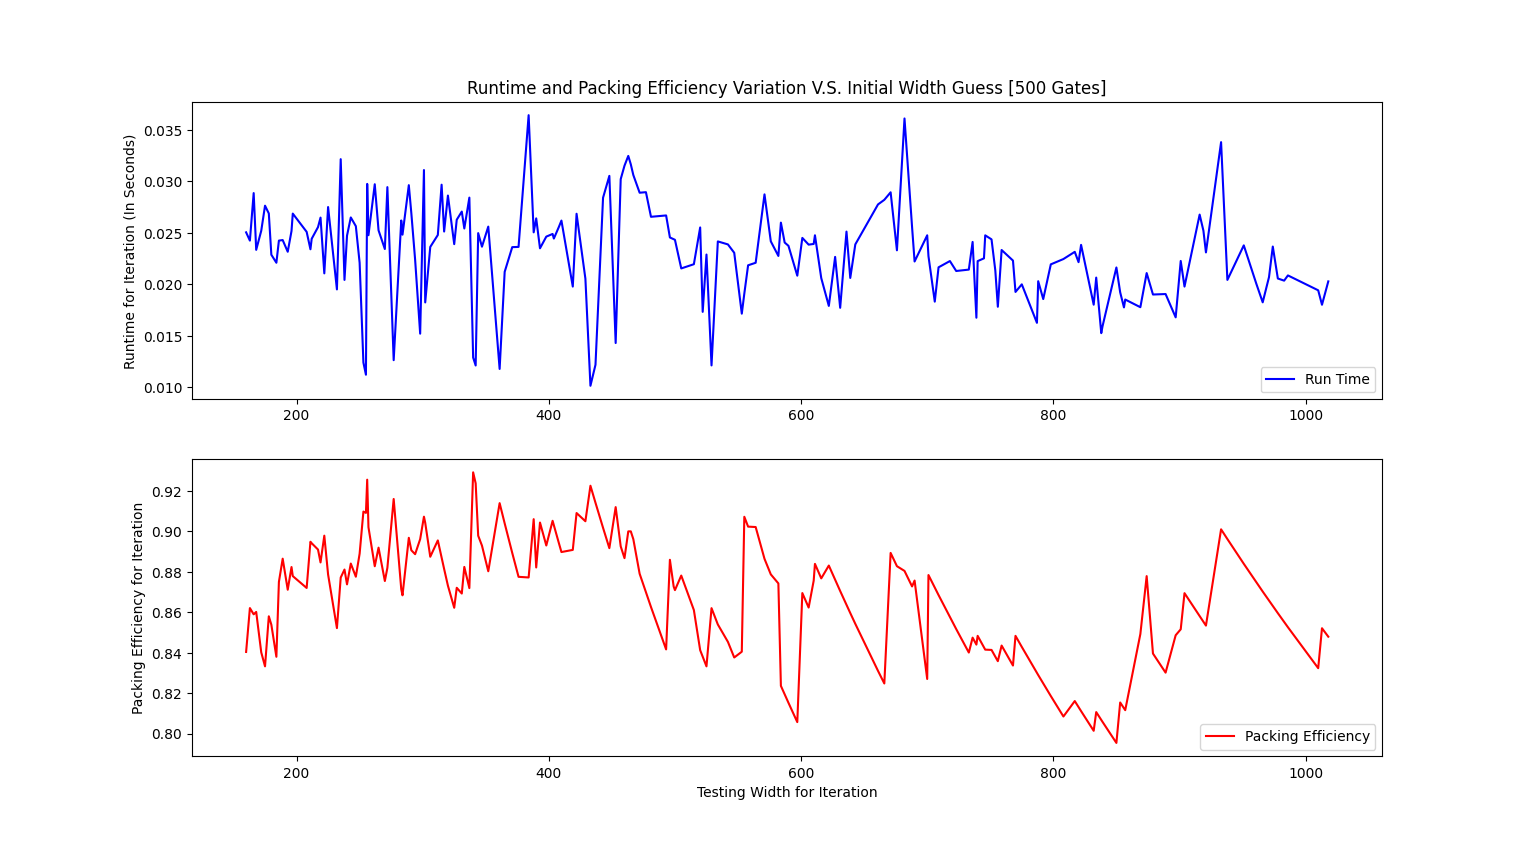
\includegraphics[width=0.9\linewidth]{Images/BRoll/Init_Width_Peff_Time_32.png}
          % \captionof{figure}{A figure}
          \label{fig:analysis-1}
          \caption{Runtime \& Packing Efficiency Variation vs Width (32 gates) }
          \centering
          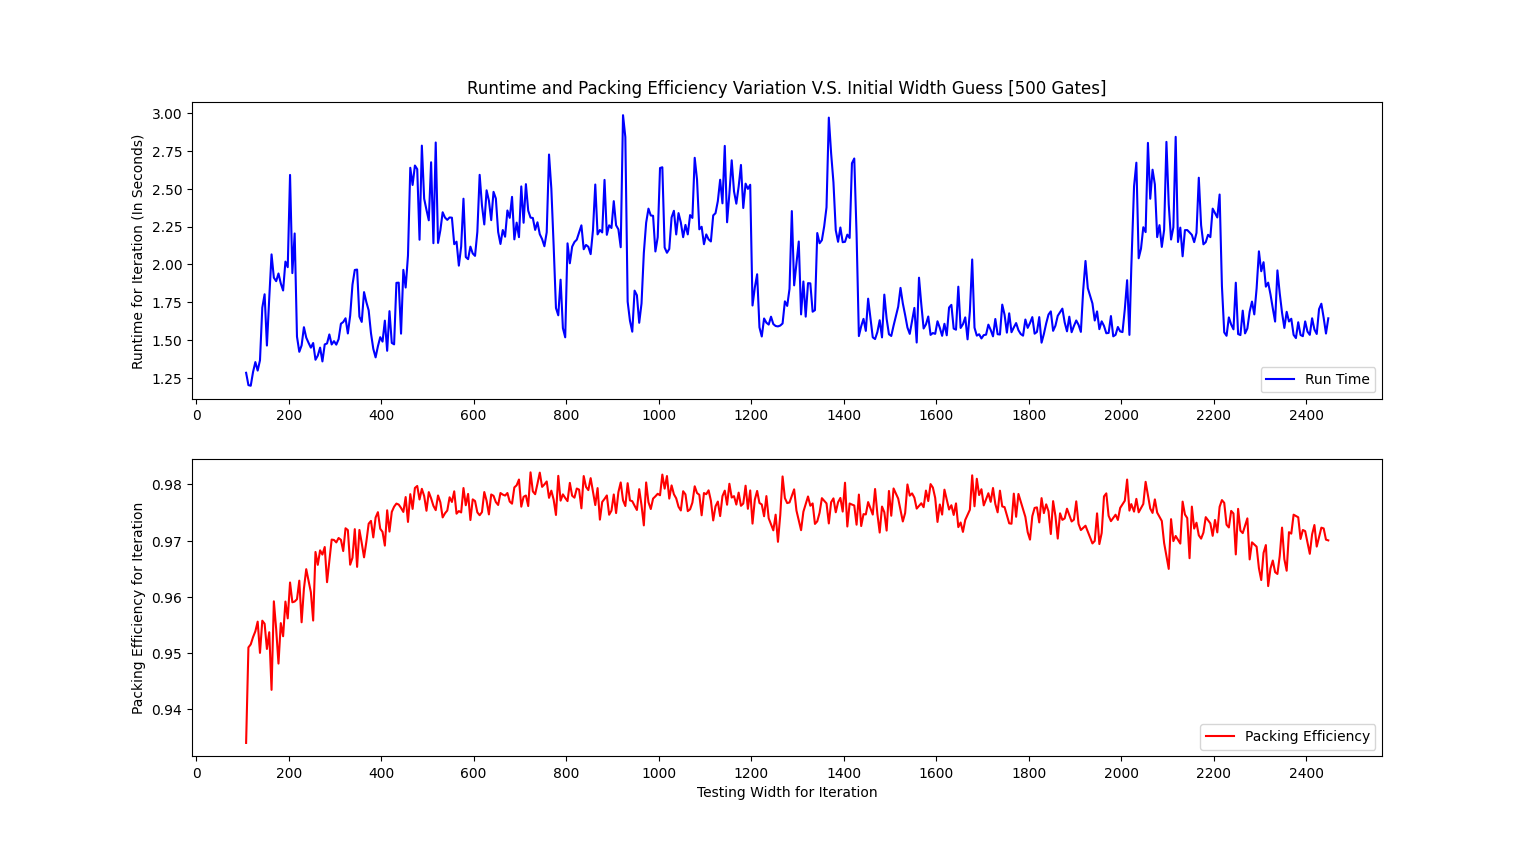
\includegraphics[width=0.9\linewidth]{Images/BRoll/Init_Width_Peff_Time_500.png}
          % \captionof{figure}{A figure}
          \label{fig:analysis-2}
          \caption{Runtime \& Packing Efficiency Variation vs Width (500 gates) }
          
               
    \end{minipage}
\end{figure}


\subsubsection{Correctness of Algorithm}
\begin{enumerate}
    \item In this variant, the small rectangles can have varying lengths and widths, and their orientation is fixed (they cannot be rotated). The goal is to pack them in an enclosing rectangle of minimum area, with no boundaries on the enclosing rectangle's width or height.The problem is NP-complete in general which means that the time required to solve the problem using any currently known algorithm increases rapidly as the size of the problem grows.
    \item The methods of solving this problem can be categorized into two types: exact algorithms and heuristic algorithms. It is well-known that the exact algorithms can only solve small-scale instances within a reasonable computational time. 
    \item Therefore, we have proposed a new heuristic rectangle packing algorithm to maximize the area usage of the box.The algorithm involves greedy placement of rectangles from large to small.
    \item If the largest rectangle remaining can't fit anywhere, we place it in a place that extends the pack region as little as possible.It is not perfect but it is easy to implement gives near perfect packing and decent runtime. 
\end{enumerate}

\begin{figure}[ht]
    \centering
    \begin{minipage}{.5\textwidth}
          \centering
          \includegraphics[width=1.0\linewidth]{Images/BRoll/complexity_classes.png}
          % \captionof{figure}{A figure}
          \label{fig:4bit-res1_sb}
          \caption{P vs NP Problems }
      
          
      \end{minipage}
    \end{figure}

%%%%%%%%%%%%%%%%%%%%%%%%%%%%%%%%%%%%%%%%%%%%%%%%%%%%%%%%%%%%%%%
\newpage % Begin Page 4 %
%%%%%%%%%%%%%%%%%%%%%%%%%%%%%%%%%%%%%%%%%%%%%%%%%%%%%%%%%%%%%%%

\section{Time Complexity Analysis}
\begin{center}
\begin{tabular}{|c|c|c|c|c|c|}
    \hline
    \rowcolor[HTML]{DAE8FC} 
    No. of rectangles & TC 1  & TC 2  &TC 3 &TC 4 &TC5 \\ \hline
    \rowcolor[HTML]{FFFC9E} 
    {Time Taken (in sec)} & {0.005484}  & {\color[HTML]{000000} 0.009657}  & {\color[HTML]{000000} 0.008263} & {\color[HTML]{000000} 0.004607}  & {\color[HTML]{000000} 0.004479}  \\ \hline
    \rowcolor[HTML]{FFFC9E} 
    {\color[HTML]{000000} Packing Efficiency}                         & {\color[HTML]{000000} 0.818181}  & {\color[HTML]{000000} 0.933333} & {\color[HTML]{000000} 0.902778}      & {\color[HTML]{000000} 0.845238}  & {\color[HTML]{000000} 0.952381}                \\ \hline
    
\end{tabular}
\end{center}
\subsection{Plot of n vs T (n is the size of the test case}

%%%%%%%%%%%%%%%%%%%%%%%%%%%%%%%%%%%%%%%%%%%%%%%%%%%%%%%%%%%%%%%%%
\newpage % Begin Page 5 %
%%%%%%%%%%%%%%%%%%%%%%%%%%%%%%%%%%%%%%%%%%%%%%%%%%%%%%%%%%%%%%%%%

\section{Visualising Output on Multiple Test Cases}

\subsection{Test Case 1}
\begin{center}
\begin{tabular}{|c|c|c|}
    \hline
    \rowcolor[HTML]{DAE8FC} Gate No. &
    Input \((w,h)\)                                    & Output \((x,y)\)   \\ \hline
    \rowcolor[HTML]{FFFC9E} {\color[HTML]{000000} \(1\)} &
    {\color[HTML]{000000} \((3,10)\)}                         & {\color[HTML]{000000} \((0,0\))}    \\ \hline
    \rowcolor[HTML]{FFFC9E} 
    {\color[HTML]{000000} \(2\)} &
    {\color[HTML]{000000} \((8,3)\)}                         & {\color[HTML]{000000} \((3,0)\)}      \\ \hline
     \rowcolor[HTML]{FFFC9E} 
     {\color[HTML]{000000} \(3\)} &
    {\color[HTML]{000000} \((6,6)\)}                         & {\color[HTML]{000000} \((3,6\))}      \\ \hline
    
\end{tabular}
\end{center}
\begin{center}
\textbf{Bounding Box Dimension : Width = \(11\) , Height = \(10\)}    
\end{center}
\begin{figure}[ht]
    \centering
    \begin{minipage}{.6\textwidth}
          \centering
          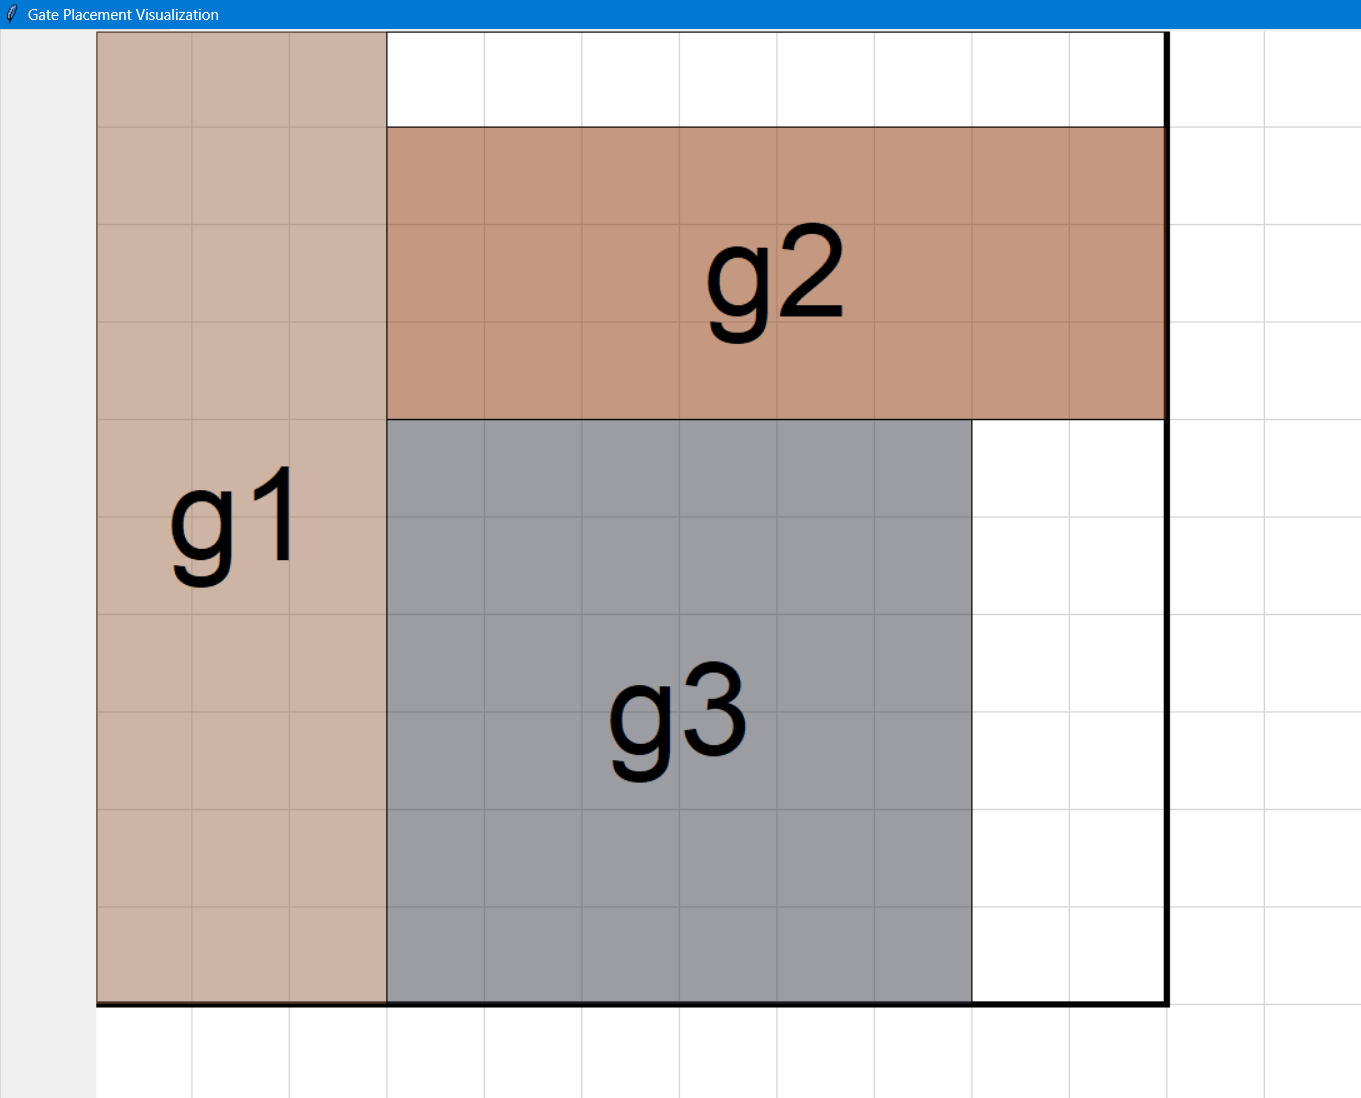
\includegraphics[width=1.0\linewidth]{Images/BRoll/Our_Packing_TC1.png}
          % \captionof{figure}{A figure}
          \label{fig:tc-1}
          \caption{Gate Packing }
      
          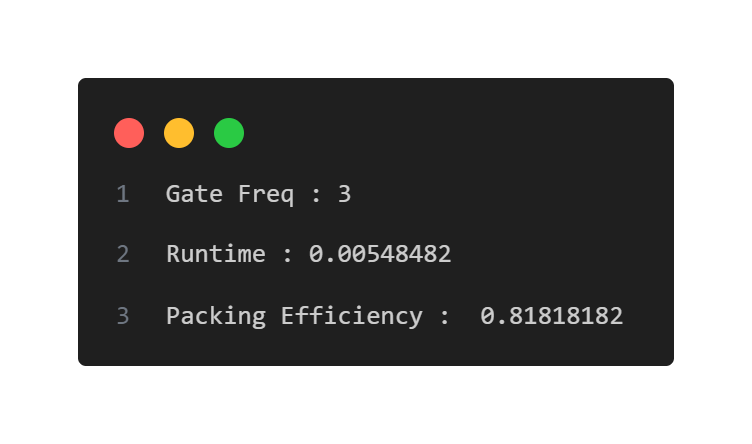
\includegraphics[width=0.95\linewidth]{Images/BRoll/Our_Packing_TC1_Report.png}
          % \captionof{figure}{A figure}
          \label{fig:tcr-1}
          \caption{Report}
          \centering 
      \end{minipage}
    \end{figure}

    
\newpage
\subsection{Test Case 2}
\begin{center}
\begin{tabular}{|c|c|c|}
    \hline
    \rowcolor[HTML]{DAE8FC} Gate No. &
    Input \((w,h)\)                                    & Output \((x,y)\)   \\ \hline
    \rowcolor[HTML]{FFFC9E} {\color[HTML]{000000}\(1\)} &
    {\color[HTML]{000000}\((3,4)\)}                         & {\color[HTML]{000000}\((0,0)\)}    \\ \hline
    \rowcolor[HTML]{FFFC9E} 
    {\color[HTML]{000000} \(2\)} &
    {\color[HTML]{000000}\((5,2)\)}                         & {\color[HTML]{000000}\((3,0)\)}      \\ \hline
     \rowcolor[HTML]{FFFC9E} 
     {\color[HTML]{000000} \(3\)} &
    {\color[HTML]{000000}\((2,3)\)}                         & {\color[HTML]{000000}\((0,4)\)}      \\ \hline
    
\end{tabular}
\end{center}
\begin{center}
\textbf{Bounding Box Dimension : Width = \(5\) , Height = \(6\)}   
\end{center}
\begin{figure}[ht]
    \centering
    \begin{minipage}{.6\textwidth}
          \centering
          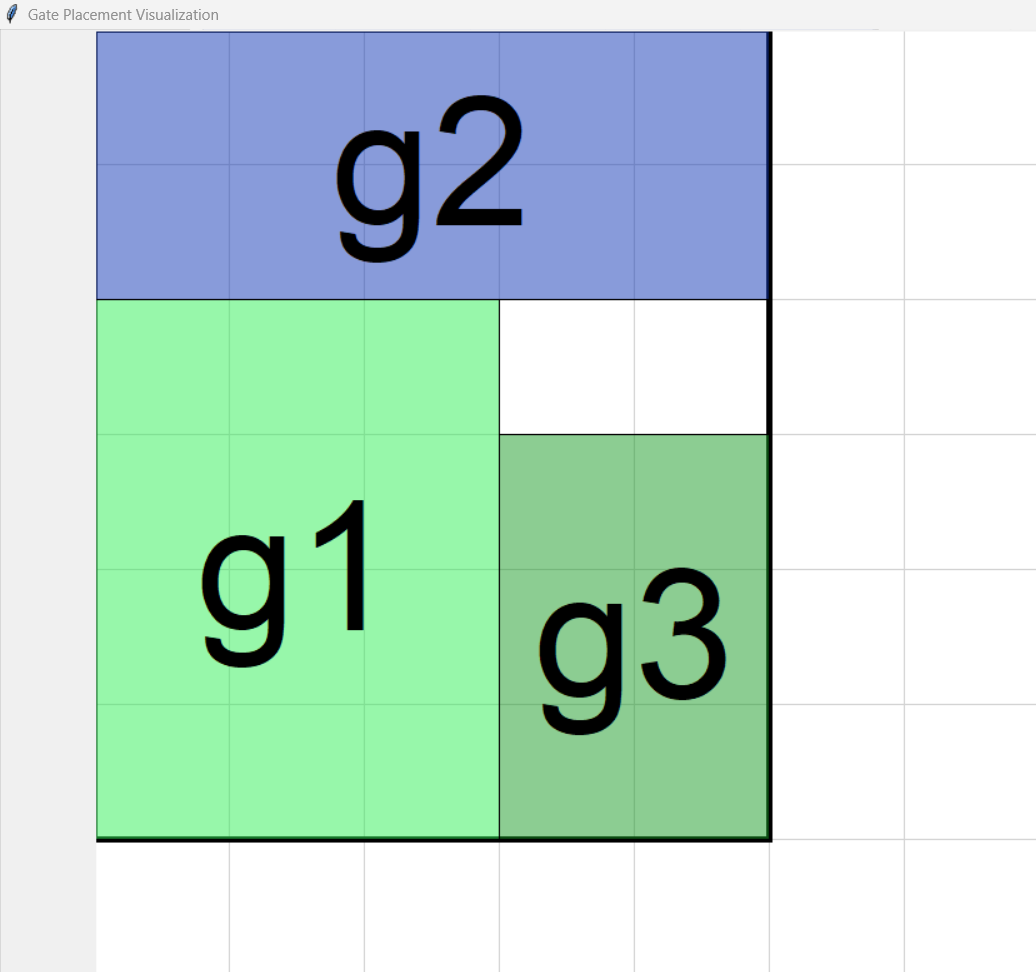
\includegraphics[width=1.0\linewidth]{Images/BRoll/Our_Packing_TC2.png}
          % \captionof{figure}{A figure}
          \label{fig:tc-2}
          \caption{Gate Packing }
     
          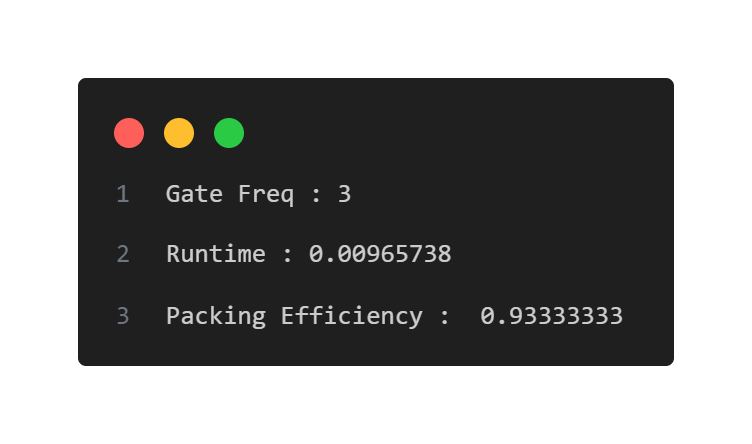
\includegraphics[width=0.95\linewidth]{Images/BRoll/Our_Packing_TC2_Report.png}
          % \captionof{figure}{A figure}
          \label{fig:tcr-2}
          \caption{Report}
    \end{minipage}
\end{figure}

    
\newpage
\subsection{Test Case 3}

\begin{center}
\begin{tabular}{|c|c|c|}
    \hline
    \rowcolor[HTML]{DAE8FC} Gate No. &
    Input \((w,h)\)                                    & Output \((x,y)\)  \\ \hline
    \rowcolor[HTML]{FFFC9E} {\color[HTML]{000000}\(1\)} &
    {\color[HTML]{000000} \((10,10)\)}                         & {\color[HTML]{000000} \((45,10)\)}    \\ \hline
    \rowcolor[HTML]{FFFC9E} 
    {\color[HTML]{000000} \(2\)} &
    {\color[HTML]{000000} \((20,5)\)}                         & {\color[HTML]{000000} \((35,25)\)}      \\ \hline
     \rowcolor[HTML]{FFFC9E} 
     {\color[HTML]{000000} \(3\)} &
    {\color[HTML]{000000} \((5,20)\)}                         & {\color[HTML]{000000} \((15,0)\)}      \\ \hline
    \rowcolor[HTML]{FFFC9E} {\color[HTML]{000000}\(4\)} &
    {\color[HTML]{000000} \((15,10)\)}                         & {\color[HTML]{000000} \((30,10)\)}    \\ \hline
    \rowcolor[HTML]{FFFC9E} 
    {\color[HTML]{000000} \(5\)} &
    {\color[HTML]{000000} \((10,15)\)}                         & {\color[HTML]{000000} \((20,0)\)}      \\ \hline
     \rowcolor[HTML]{FFFC9E} 
     {\color[HTML]{000000} \(6\)} &
    {\color[HTML]{000000} \((25,5)\)}                         & {\color[HTML]{000000} \((10,25)\)}      \\ \hline
    \rowcolor[HTML]{FFFC9E} {\color[HTML]{000000}\(7\)} &
    {\color[HTML]{000000} \((5,25)\)}                         & {\color[HTML]{000000} \((100,0)\)}    \\ \hline
    \rowcolor[HTML]{FFFC9E} 
    {\color[HTML]{000000} \(8\)} &
    {\color[HTML]{000000} \((30,10)\)}                         & {\color[HTML]{000000} \((30,0)\)}      \\ \hline
     \rowcolor[HTML]{FFFC9E} 
     {\color[HTML]{000000} \(9\)} &
    {\color[HTML]{000000} \((10,30)\)}                         & {\color[HTML]{000000} \((0,0\))}      \\ \hline
    \rowcolor[HTML]{FFFC9E} {\color[HTML]{000000}\(10\)} &
    {\color[HTML]{000000} \((35,5)\)}                         & {\color[HTML]{000000} \((15,20)\)}    \\ \hline
    
    
\end{tabular}
\end{center}
\begin{center}
\textbf{Bounding Box Dimension : Width = \(60\) , Height = \(30\)}     
\end{center}

\begin{figure}[ht]
    \centering
    \begin{minipage}{.6\textwidth}
          \centering
          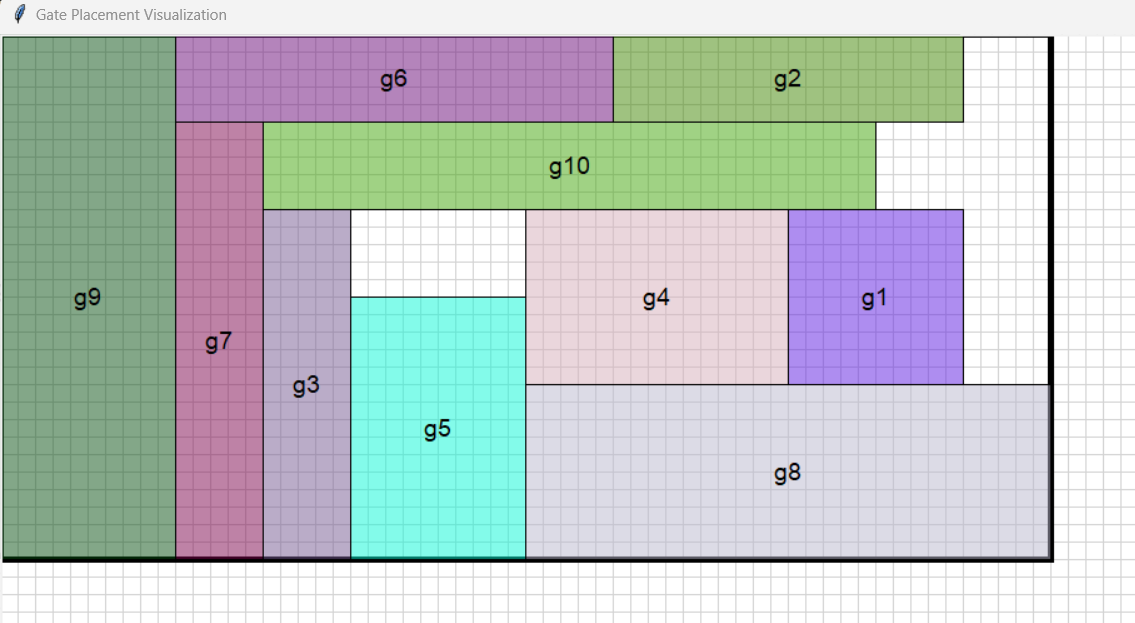
\includegraphics[width=1.0\linewidth]{Images/BRoll/Our_Packing_TC3.png}
          % \captionof{figure}{A figure}
          \label{fig:tc-3}
          \caption{Gate Packing }
      
          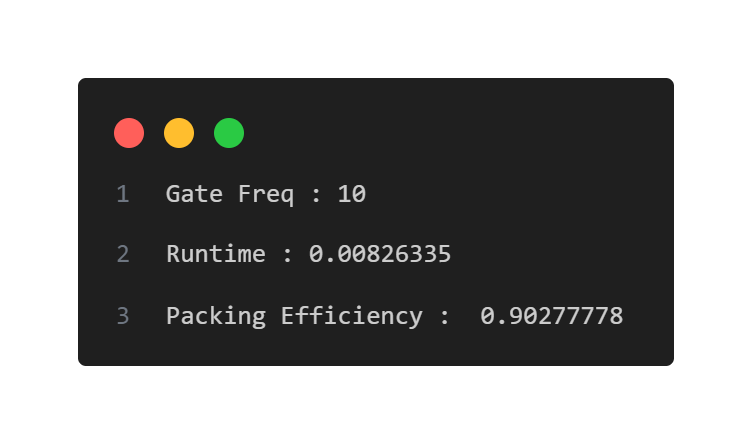
\includegraphics[width=0.95\linewidth]{Images/BRoll/Our_Packing_TC3_Report.png}
          % \captionof{figure}{A figure}
          \label{fig:tcr-3}
          \caption{Report}
          \centering 
      \end{minipage}
    \end{figure}

\newpage
\subsection{Test Case 4}
\begin{center}
\begin{tabular}{|c|c|c|}
    \hline
    \rowcolor[HTML]{DAE8FC} Gate No. &
    Input (w,h)                                    & Output(x,y)   \\ \hline
    \rowcolor[HTML]{FFFC9E} {\color[HTML]{000000}\(1\)} &
    {\color[HTML]{000000} \((4,5)\)}                         & {\color[HTML]{000000} \((2,0)\)}    \\ \hline
    \rowcolor[HTML]{FFFC9E} 
    {\color[HTML]{000000} \(2\)} &
    {\color[HTML]{000000} \((6,2\))}                         & {\color[HTML]{000000} \((6,4)\)}      \\ \hline
     \rowcolor[HTML]{FFFC9E} 
     {\color[HTML]{000000} \(3\)} &
    {\color[HTML]{000000} \((6,0)\)}                         & {\color[HTML]{000000} \((0,0)\)}      \\ \hline
      \rowcolor[HTML]{FFFC9E}  {\color[HTML]{000000}\(4\)} &
    {\color[HTML]{000000} \((3,4)\)}                         & {\color[HTML]{000000} \((6,0)\)}      \\ \hline
     \rowcolor[HTML]{FFFC9E} 
     {\color[HTML]{000000} \(5\)} &
    {\color[HTML]{000000} \((5,3)\)}                         & {\color[HTML]{000000} \((9,0)\)}      \\ \hline
    
    
\end{tabular}
\end{center}
\begin{center}
\textbf{Bounding Box Dimension : Width = \(14\) , Height = \(6\)} 
\end{center}

\begin{figure}[ht]
    \centering
    \begin{minipage}{.6\textwidth}
          \centering
          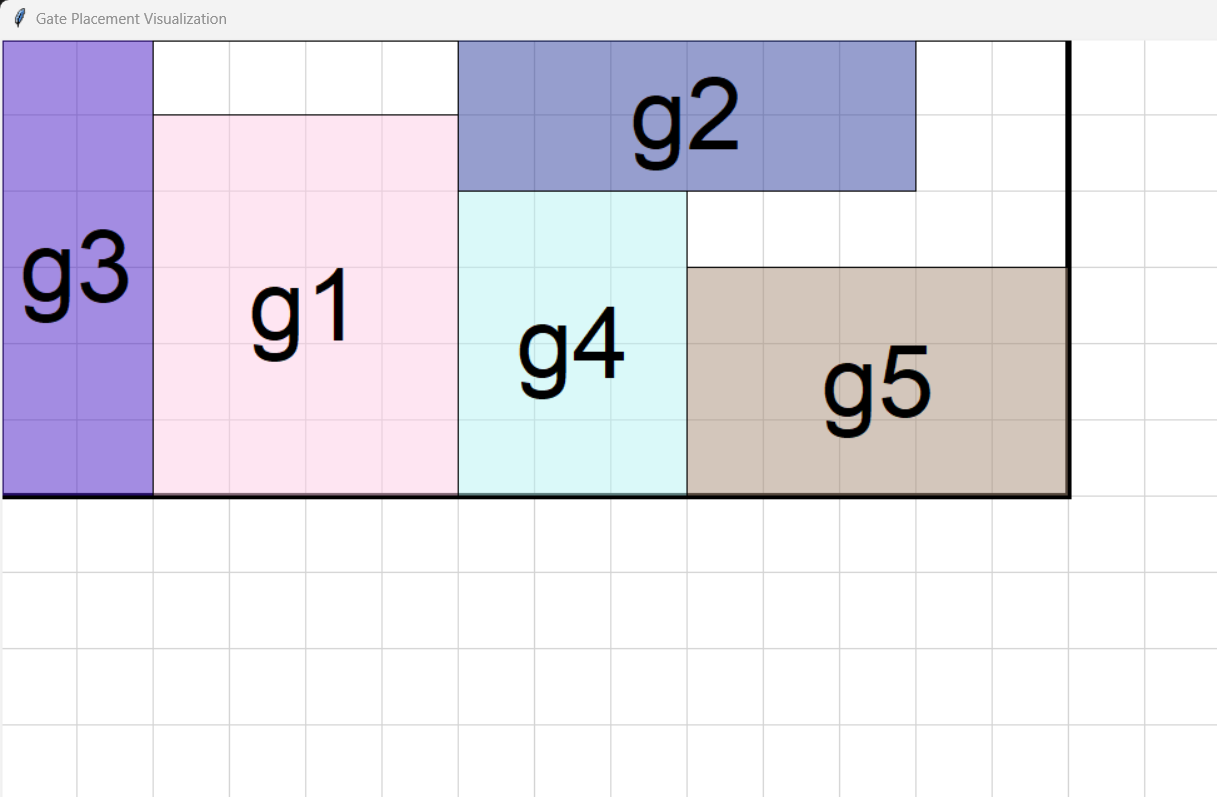
\includegraphics[width=1.0\linewidth]{Images/BRoll/Our_Packing_TC4.png}
          % \captionof{figure}{A figure}
          \label{fig:tc-4}
          \caption{Gate Packing }
     
          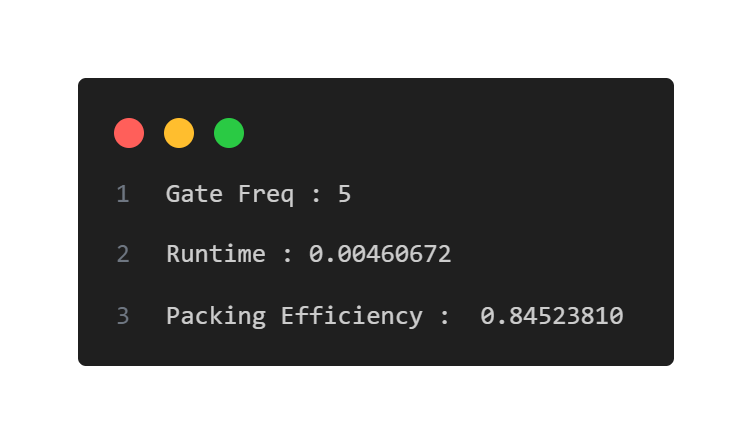
\includegraphics[width=0.95\linewidth]{Images/BRoll/Our_Packing_TC4_Report.png}
          % \captionof{figure}{A figure}
          \label{fig:tcr-4}
          \caption{Report}
          \centering 
      \end{minipage}
    \end{figure}

\newpage
\subsection{Test Case 5}
\begin{figure}[ht]
    \centering
    \begin{minipage}{.7\textwidth}
          \centering
          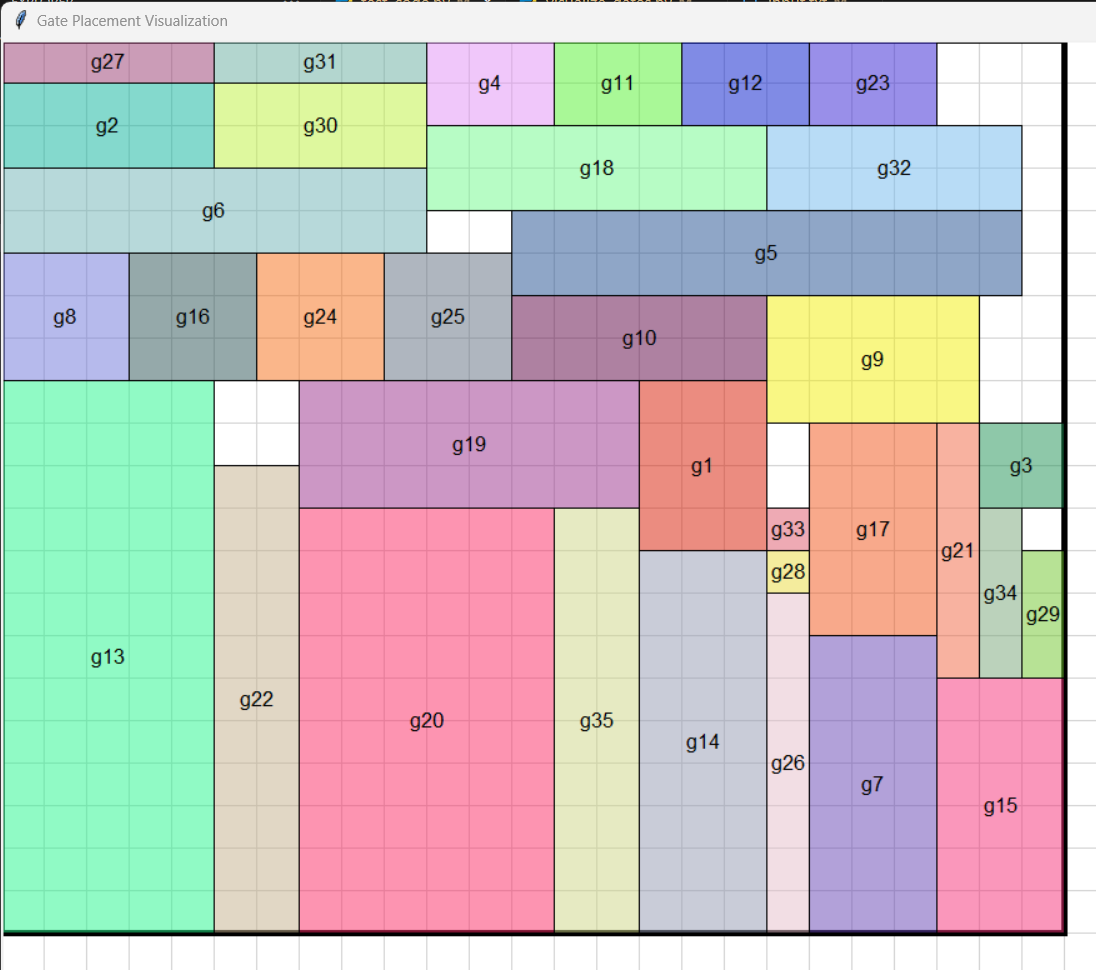
\includegraphics[width=1.0\linewidth]{Images/BRoll/output_sample_tc5.png}
          % \captionof{figure}{A figure}
          \label{fig:tc-5}
          \caption{Gate Packing }
      
          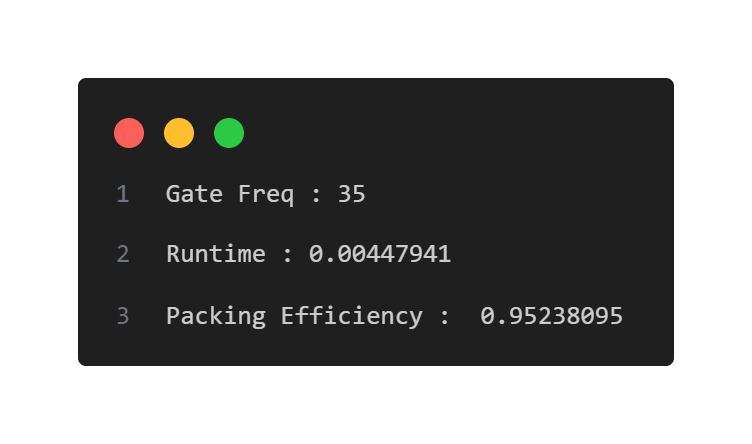
\includegraphics[width=0.95\linewidth]{Images/BRoll/Our_Packing_TC5_Report.png}
          % \captionof{figure}{A figure}
          \label{fig:tcr-5}
          \caption{Report}
          \centering 
      \end{minipage}
\end{figure}



\end{document}